\section{Organisation générale}
\subsection{Enseignants}
Enseignants en PTSI 1 : Xavier PESSOLES \url{xpessoles@lamartin.fr} et Isabelle COTTA \url{cotta.PTSI1@gmail.com}.

Enseignants en PTSI 2 : Xavier PESSOLES \url{xpessoles@lamartin.fr} et Viviane REYDELLET \url{viviane.reydellet.m@gmail.com}.

\subsection{Sites Internet}

Le site dédié à l'informatique en PTSI est le suivant :
\url{https://ptsilamartin.github.io/info.html}

\textbf{Vous trouverez sur ce site un chapitre {Activités}. Avant chaque TP une activité préparatoire est à réaliser impérativement. Le lien sera dans le chaptre Activité et vous renverra sur Capytale. Pour se connecter, il faut disposer d'un compte Educonnect.}


Vous pouvez aussi trouver des informations sur mon site personnel \url{xpessoles-cpge.fr}.
\section{Programmation en Python}
\subsection{Cahiers (Notebooks) en ligne}

\url{https://capytale2.ac-paris.fr/} est une interface en ligne pour programmer en Python.
Il faut se rendre sur le site, choisir l'ENT \textbf{Ma Classe en Région (Auvergne-Rhône-Alpes)} et utiliser vos identifiants EduConnect pour se connecter.

Vous y trouverez des travaux à réaliser en autonomie.

\begin{center}
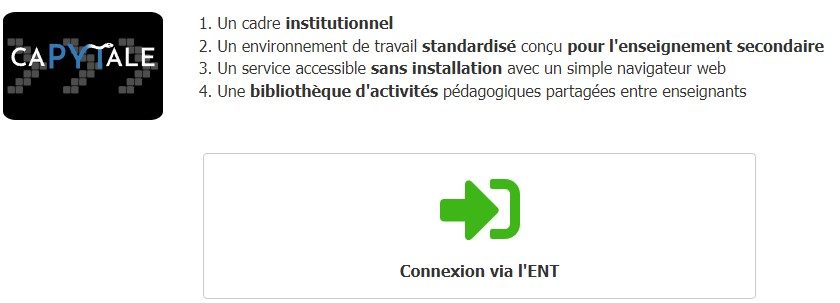
\includegraphics[scale=0.4]{capytale.jpg}
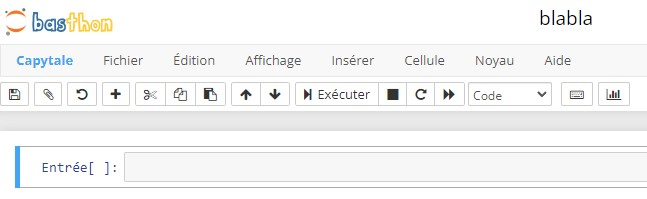
\includegraphics[scale=0.4]{capytale2.jpg}
\end{center}

\subsection{Environnmenet de programmation}

L'environnement de développement (IDE) utilisé au lycée pour programmer en Pyhon est \texttt{Pyzo}.

Pour programmer en Python sur votre ordinateur personnel vous avez besoin d'une distribution Python (par exemple Anaconda) et d'un environnement de développent (PYZO).
Rendez-vous sur le site \url{Pyzo.org} qui vous propose une fenêtre \texttt{Quickstart}.\\
L'installation se fait en quatre temps selon les éléments choisis :
\begin{enumerate}
\item Installation de l'IDE, choisir la version correspondant à votre système d'exploitation (Windows, MacOS, Linux) \url{https://github.com/pyzo/pyzo/releases/download/v4.16.0/pyzo-4.16.0-win64.exe} pour Windows.
\item Installer la distribution \texttt{Anaconda}.
\item Configurer votre shell au lancement de \texttt{Pyzo} la première fois dans la fenêtre en haut à gauche .

\begin{center}
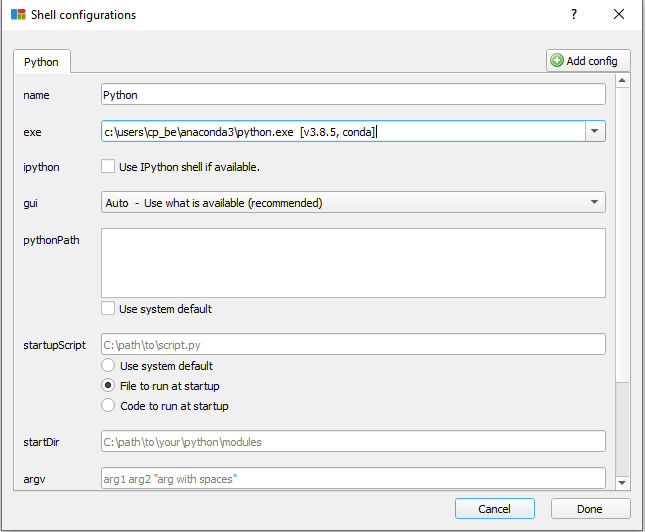
\includegraphics[scale=0.6]{Capture.png}
\end{center}

\item Les bibliothèques nécessaires sont installées par défaut si vous avez installé anaconda, l'étape 4 n'est pas utile. Sauf si vous avez dû installer une distribution plus légère.
\end{enumerate}






\subsubsection{Changement de thème de la fenêtre Pyzo}
Si l'écran blanc de la fenêtre \texttt{Pyzo} fatigue vos yeux, vous pouvez le changer :\\
setting $\backslash$ edit syntax styles... $\backslash$ \\
Vous pouvez choisir \texttt{solarized\_dark}.


\subsubsection{IDLE python}
Vous serez amené en math-info à utiliser l'IDLE Python aussi installé sur les ordinateurs du lycée.\\
Moins convivial que \texttt{Pyzo}, il permet de réaliser les mêmes travaux en utilisant les deux types de fenêtres celle du \texttt{shell} (ou \texttt{console}) et celle d'\texttt{édition}.

\begin{center}
\includegraphics[scale=0.6]{idleRunScript.png}
\end{center}

%Rendez-vous sur le site \texttt{Python.org} et choisissez votre système d'exploitation.\\
%Les deux versions \texttt{IDLE Python} et \texttt{Pyzo} peuvent être installées sur votre ordinateur sans conflit.\\
%Les bibliothèques ne sont pas installées par défaut.

L'\texttt{IDLE Python} est disponible avec toute installation de Python. Avec Pyzo, aller dans dossier contenant Pyzo ou Anaconda puis dans le répertoire \texttt{Lib\textbackslash idlelib} et lancer le programme \texttt{idle.bat}.\\
Le chemin peut être celui-ci \texttt{C:\textbackslash Users\textbackslash ...\textbackslash anaconda3\textbackslash Lib\textbackslash idlelib} par exemple.

\subsection{Python via des notebook : Jupyter, Capytale, Google Colab}

\subsection{Jupyter}
\texttt{Jupyter.org} est accessible par votre moteur de recherche préféré.\\
Je vous propose : \texttt{Try Jupyter} puis \texttt{JupyterLab}

\begin{center}
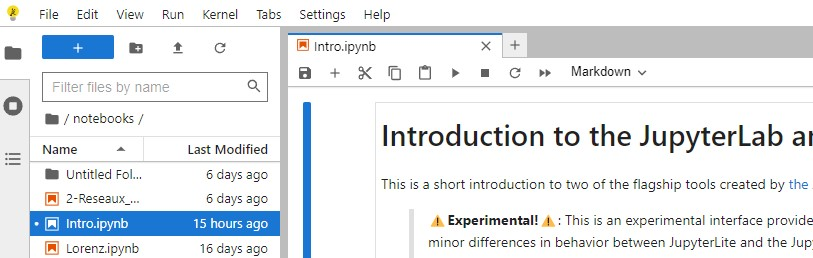
\includegraphics[scale=0.4]{jupyter.jpg}
\end{center}

Ouvrir une page vierge avec le \textbf{+} de l'onglet et sélectionner \texttt{notebook} et \texttt{Python}.


\begin{center}
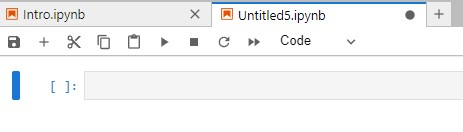
\includegraphics[scale=0.6]{jupyter2.jpg}
\end{center}

Vous pouvez écrire des lignes de codes dans la case et les exécuter avec la flèche.


